\begin{frame}
  \frametitle{The delayed neutron count rate is dominated by a few DNPs}
        \begin{columns}
                \column[t]{0.5\textwidth}
        \begin{figure}[htbp!]
        \begin{center}
        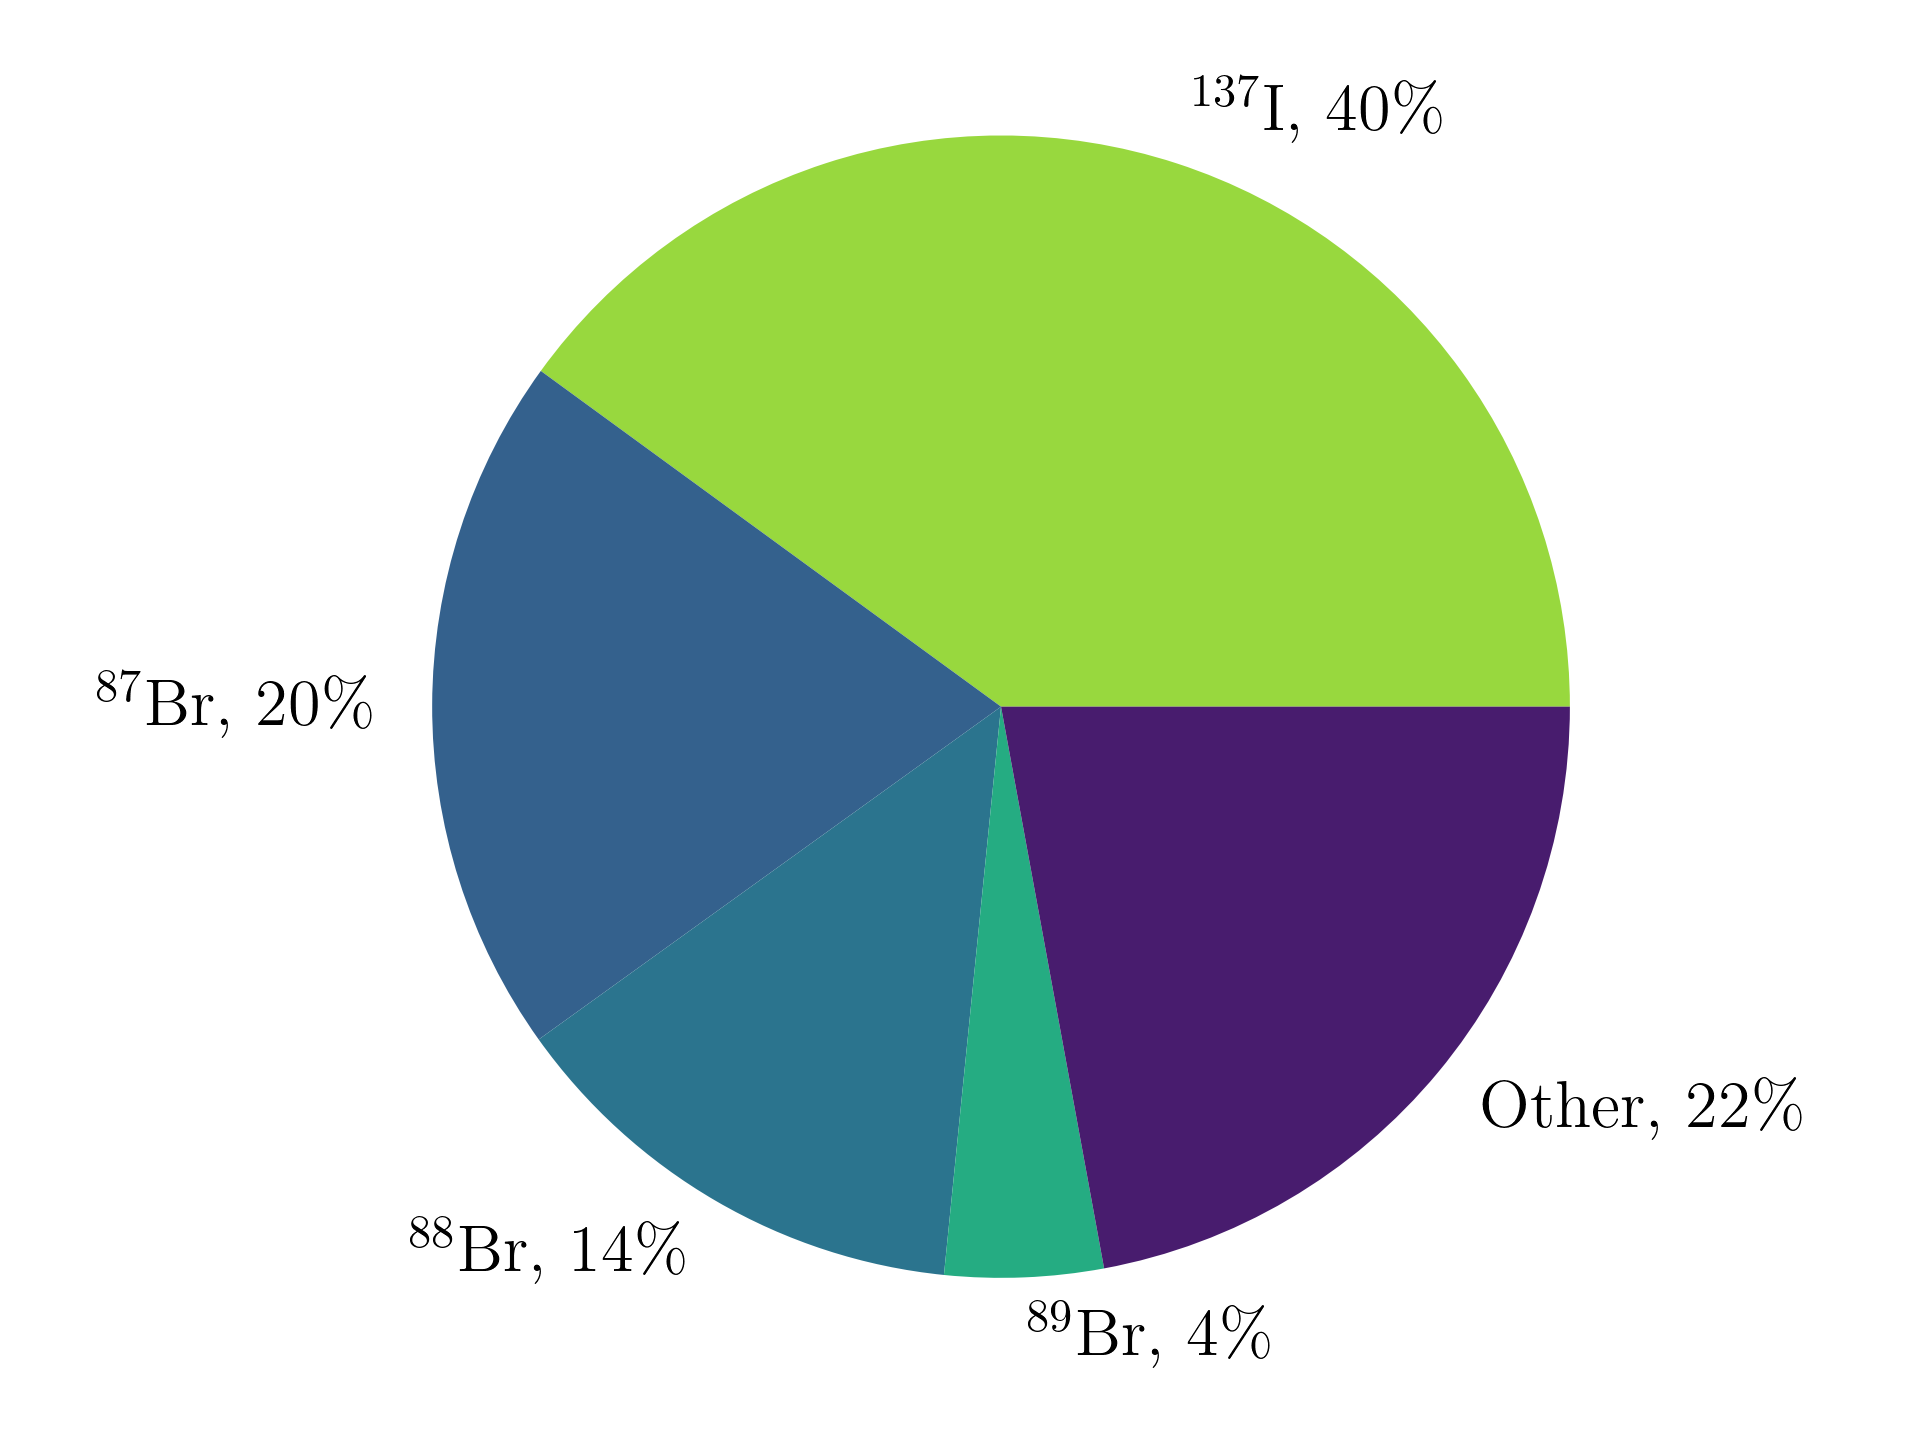
\includegraphics[width=1\textwidth]{../images/1dnp_yield.png}
        \end{center}
            \caption{Relative delayed neutron counts from each \gls{DNP} after a thermal saturation irradiation of $^{235}$U using the 0D scaled model.}
        \end{figure}

                \column[t]{0.5\textwidth}
        \begin{figure}[htbp!]
        \begin{center}
        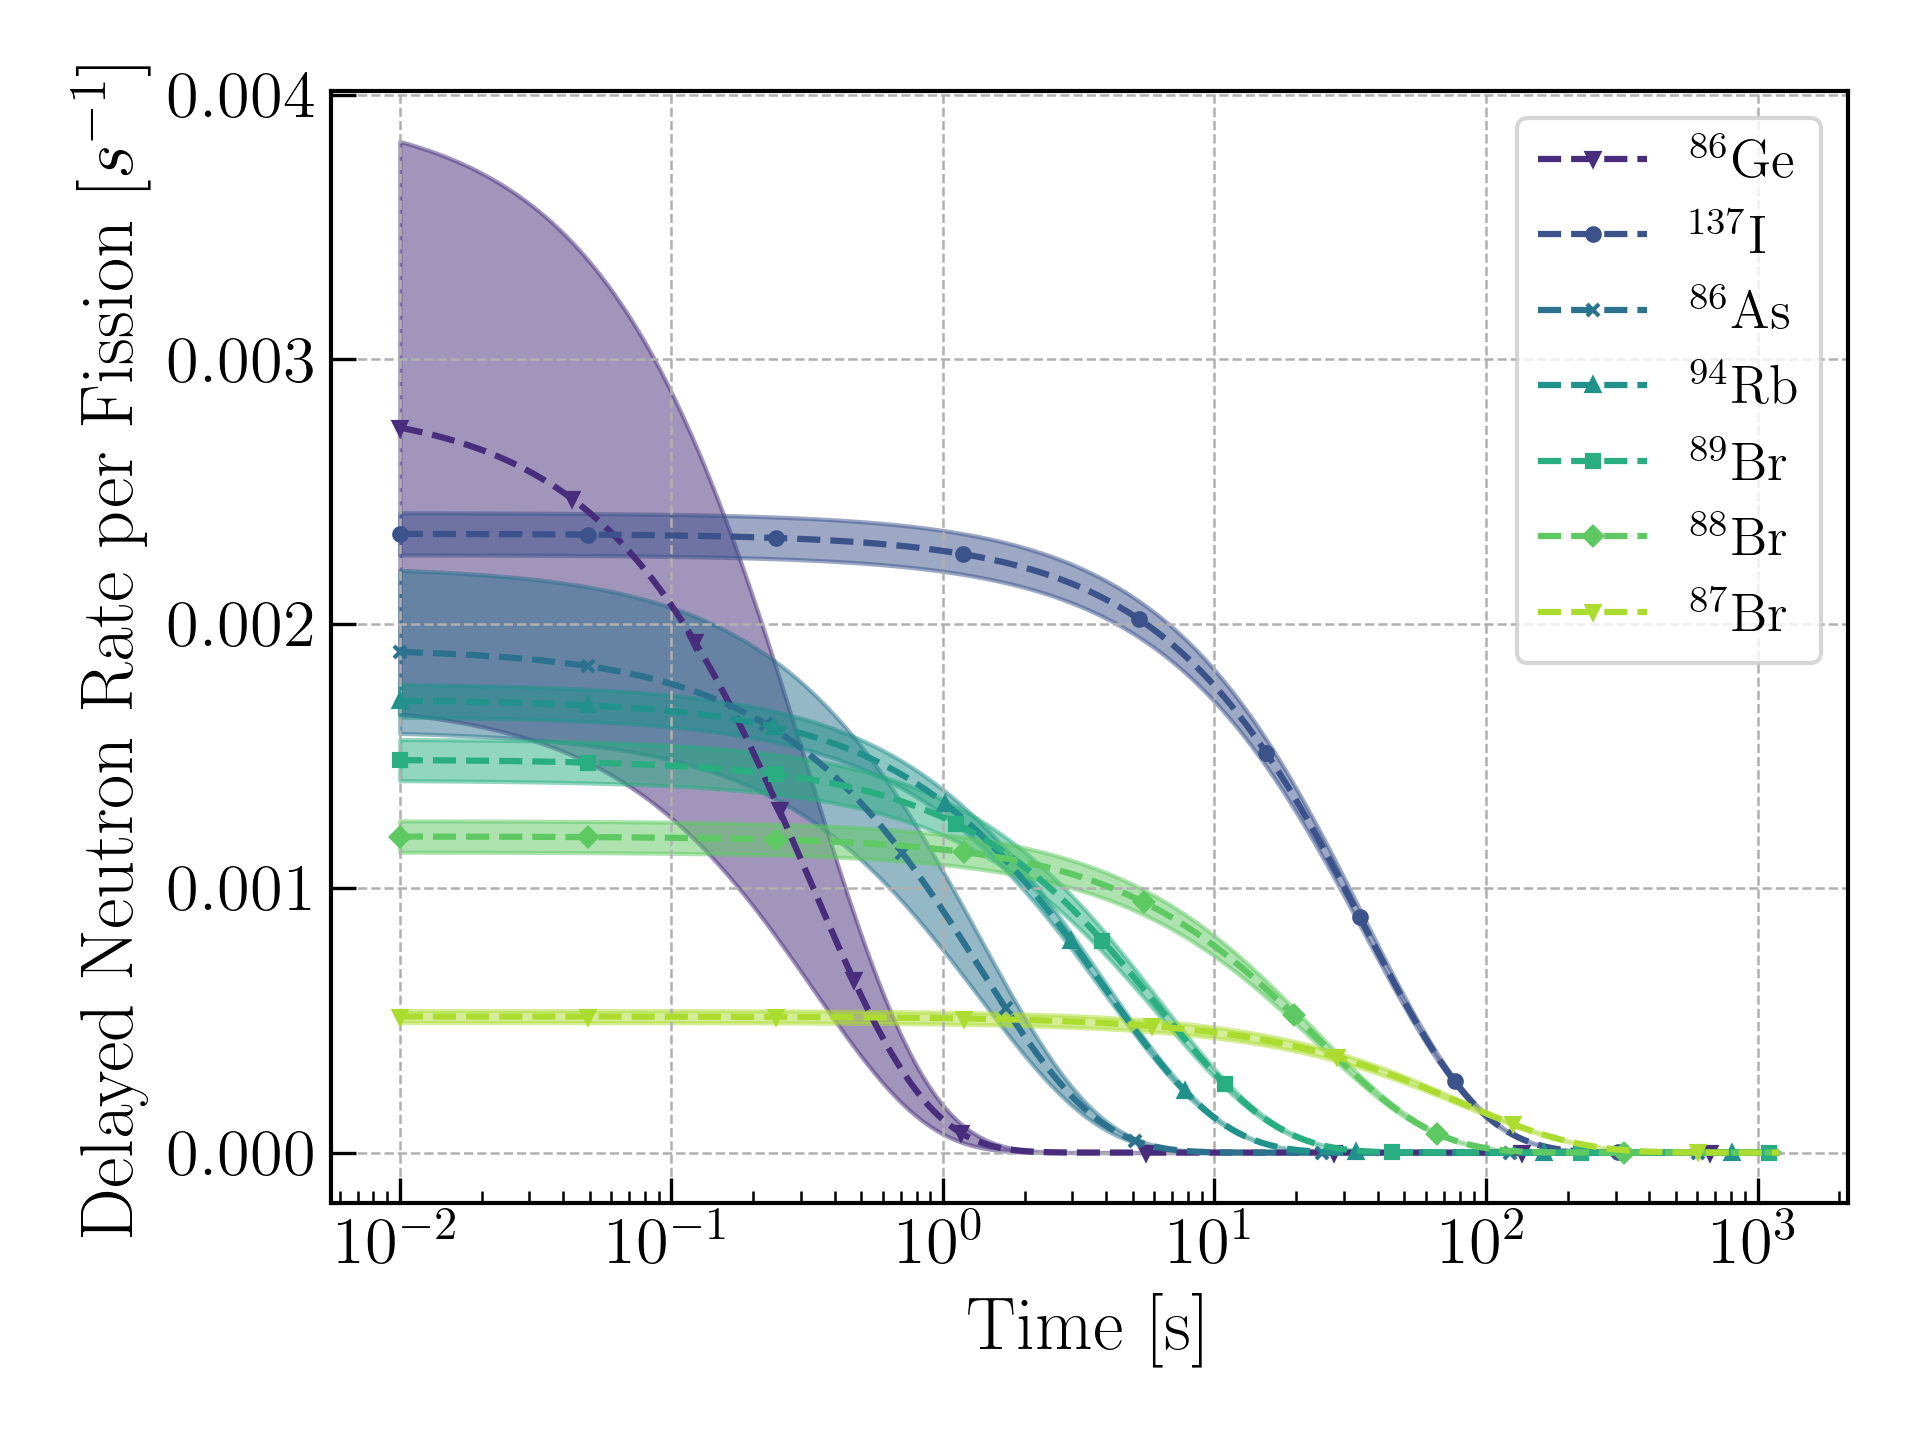
\includegraphics[width=1\textwidth]{../images/individual_nuclide_rates.png}
        \end{center}
            \caption{Relative delayed neutron count rates after a thermal saturation irradiation of $^{235}$U using the 0D scaled model.}
        \end{figure}
        \end{columns}
\end{frame}
